\subsection{Interessentanalyse}
Dette afsnit vil undersøge hvilke interessenter der er, og hvilken interesse de har i problemet og en eventuel løsning af problemet. Vi har udvalgt fem interessenter ud fra emnet lamper, da belysning fra lamper er det centrale i det initierende problem. Formålet med interessentanalysen er at finde ud af hvilke interessenter som denne rapport vil løse problemet for.

[Indledning til designere, producenter, lampebutikker og brugere]
\begin{figure}[H]
	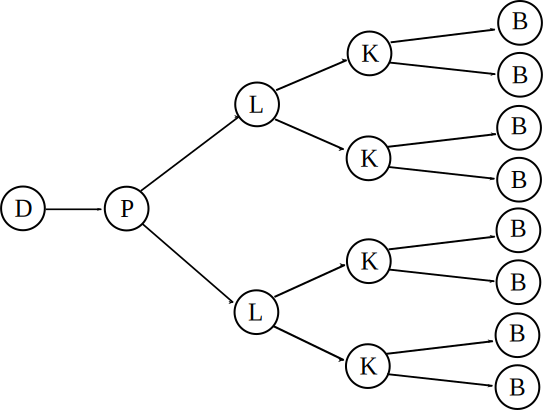
\includegraphics[width=\textwidth]{interessenter.pdf}
	\caption{De fem interessenters forbindelse.}
    \label{fig:interessenter}
\end{figure}
% Sælgeren bliver også indirekte ramt, hvis mange kunder henvender sig fordi de gerne vil have en lampe returneret og byttet, så kræver det ressourcer fra lampebutikkers side. Derfor vil det også være til lampebutikkers fordel, at en kunde vil være i stand til at købe "den rigtige" lampe første gang eller en lampe, der er lidt dyrere fordi den giver den ønskede effekt.

\subsubsection{Designere}
Designere er interesseret i at deres design bliver solgt og er derfor sandsynligvis interesseret i et program der kan hjælpe dem med at gøre deres design mere populært.
Vi har haft kontakt til en lampedesigner fra IKEA Sverige, som fortalte os at de bruger et program kaldet "Solid Works"\cite{SolidWorks} til at designe lamper og renderer deres design, men bruger prototyper til at visualiserer lyset fra lampen\cite{sec:mailDavid}.
Vi har også haft kontakt med Erik Mortensen som er dansk lampedesigner og fortæller at lysforholdene er 2. prioritet og først afgøres ved hjælp af prototyper når resten af lampen er designet\cite{sec:mailErik}.

\subsubsection{Producenter}
Producenten samarbejder med designeren om at udvikle lampen. Producentens rolle er at fremstille lampen på baggrund af designet. Når lamperne er produceret sendes de ud til lampebutikkerne. Producenten kan have en interesse i, at kunderne køber deres produkter i lampebutikkerne, da dette højst sandsynligt vil medføre at lampebutikkerne bestiller flere af deres produkter hjem. 

\subsubsection{Lampebutikker}
Lampebutikken er interesseret i at sælge flest mulige lamper, da dette fører til større indkomst for butikken. Derudover er butikken også interesseret i, at kunden køber den 'rigtige' lampe første gang, da butikken på denne måde undgår utilfredse kunder, som vil returnere lamperne.

\subsubsection{Kunder}
Kunden er interesseret i at visualisere hvordan lys udbreder sig fra en lampe, da dette vil hjælpe kunden med at afgøre hvordan lampen passer ind i en kontekst, og kunden kan derfor undgå fejlkøb. Dette er kunden interesseret i, da det i sidste evne vil gavne brugeren af lampen, hvis kunden er i stand til at købe en lampe som passer ind i konteksten.

\subsubsection{Brugere}
Det er brugerne der i sidste ende benytter sig af lamperne i deres hjem eller på deres arbejde. Dette gør brugerne til den gruppe af interessenter, som påvirkes direkte af problemet, da de må leve med konsekvenserne, som belysningen fra en lampe kan medføre[HENVIS TIL AFSNIT OM KONSEKVENSER VED LYS]. Dette kan bl.a. være kontorarbejdere i en virksomhed, som påvirkes, hvis lamperne på deres kontor ikke passer sammen med den indretning der. Et andet eksempel på brugere, er hjemme i privaten, hvor der kan være mange forskellige typer lamper, som skal passe ind i hjemmet. Hvis en person i hjemmet køber en lampe, som har en belysning, der ikke passer ind i hjemmet pga. manglende visualisering ved købet, så vil dette påvirke brugerne i hjemmet. 

\subsubsection{Målgruppen}
Som beskrevet i forrige afsnit, er det både designere, producenter, butikker, kunder og brugere, der påvirkes af problemet. Det er nu relevant at afgøre hvem problemløsningen retter sig mod, da dette danner grundlag for hvordan løsningen skal udvikles og hvem der kan indrages i løsningen og udarbejdelsen af løsningsforslaget.

Som der ses på ovenstående skitse er det lampebutikkerne, som har den direkte kontakt til kunderne og derved også forbrugerne. Designere er fravalgt, da vi ud fra mails fra Wahl og Mortensen kan uddrage, at de allerede har værktøjer til at visualisere lys fra lamper, og som der ses på skitsen har designeren ikke nogle direkte kontakt til kunden eller brugeren. Man kunne forestille sig, at problemet kunne løses allerede fra producentens side af, men ud fra vores korrespondance med en belysningskonsulent i en lampebutik er vi blevet informeret om, at producenterne ikke er interesseret i at bruge ressourcer på at løse problemet, da det ikke gavner producenterne direkte. Derudover kan vi se på skitsen at producenterne ikke har direkte kontakt med kunden eller brugeren.

Hvis man derimod retter problemløsningen mod lampebutikker, og laver en løsning der gør det muligt for kunder at visualisere lamperne bedre, så vil kunderne højst sandsynligt være mere tilfredse med deres lamper, da de har mulighed for at se lampens belysning inden købet. For lampebutikker vil dette betyde, at kunden ikke vil returnere lige så mange lamper, og dette vil bidrage til øget kundetilfredshed, som i sidste ende gavner både lampebutikker og kunderne.

\subsubsection*{Opsummering}
I afsnittet er der blevet argumenteret for, at det er lampebutikker og brugere der bliver ramt af problemet, men at det vil være mest fordelagtigt at rette løsningen mod lampebutikker, da dette også løser problemet for brugerne.

Dette afsnit er relevant i forhold til den senere problemformulering, da der er blevet argumenteret for hvem det er, som har problemet, samt hvilken målgruppe det senere produkt skal udvikles til.
